\section{Baseline Allocation Results}

\subsection{Optimization Problem Formulation}

We formulate the resource allocation problem as a constrained optimization:

\begin{equation}
\max_{x \in \mathcal{X}} \quad \mathcal{P}_{system} = \frac{\sum_{i} w_i \cdot P_i(x)}{\sum_{i} w_i}
\label{eq:optimization_obj}
\end{equation}

subject to:
\begin{align}
\sum_{k \in K} c_k x_k &\leq B \label{eq:budget_constraint} \\
\sum_{i \in \mathcal{L}} x_{ik} &\leq T_k \quad \forall k \in K \label{eq:time_constraint} \\
P_i(x) &\geq \tau_{min} \quad \forall i \in \mathcal{L}_{high} \label{eq:min_protection}
\end{align}

where:
\begin{itemize}
\item $x_{ik}$: Allocation of asset $k$ to location $i$
\item $c_k$: Unit cost of asset $k$
\item $B$: Total budget constraint
\item $T_k$: Total available time for asset $k$
\item $\mathcal{L}_{high}$: High-priority locations
\end{itemize}

\subsection{Solution Method: Genetic Algorithm with Priority Weighting}

We employ a genetic algorithm (GA) with priority-weighted fitness function:

\begin{algorithm}[H]
\caption{Priority-Weighted Allocation GA}
\begin{algorithmic}[1]
\STATE Initialize population of allocation strategies
\FOR{generation = 1 to maxGenerations}
    \FOR{each individual in population}
        \STATE Compute fitness: $F = \sum_i w_i \cdot P_i(x)$
    \ENDFOR
    \STATE Select top performers (tournament selection)
    \STATE Apply crossover (priority-preserving recombination)
    \STATE Apply mutation (random reallocation, 5\% probability)
    \STATE Elitism: retain best 10\% unchanged
\ENDFOR
\STATE Return best allocation strategy
\end{algorithmic}
\end{algorithm}

\subsection{Baseline Results: Strategic vs. Uniform}

\begin{table}[H]
\centering
\caption{Baseline Allocation Performance}
\begin{tabular}{lccc}
\toprule
\textbf{Metric} & \textbf{Uniform} & \textbf{Strategic} & \textbf{Improvement} \\
\midrule
System-Level Protection & 0.68 & \textbf{0.91} & +34\% \\
High-Priority Species Protection & 0.62 & \textbf{0.89} & +27 pp \\
Critical Area Coverage & 0.58 & \textbf{0.94} & +36 pp \\
Threat Detection Rate & 0.55 & \textbf{0.81} & +26 pp \\
Ranger Efficiency (km$^2$/ranger) & 180 & \textbf{320} & +78\% \\
Asset Utilization Rate & 0.72 & \textbf{0.89} & +17 pp \\
\bottomrule
\end{tabular}
\end{table}

\subsection{Resource Allocation Breakdown}

\begin{table}[H]
\centering
\caption{Strategic Allocation Distribution}
\begin{tabular}{lcc}
\toprule
\textbf{Resource Type} & \textbf{High-Priority Zones} & \textbf{Medium-Priority Zones} \\
\midrule
Ranger Patrols & 65\% & 25\% \\
UAV Surveillance & 25\% & 45\% \\
Camera Traps & 10\% & 30\% \\
\bottomrule
\end{tabular}
\end{table}

\noindent \textbf{Key Insight:} High-priority zones receive concentrated ranger presence (deterrence through visible presence), while medium-priority zones rely on technological monitoring (cost-effective surveillance).

\subsection{Geographic Distribution of Protection}

\begin{figure}[H]
\centering
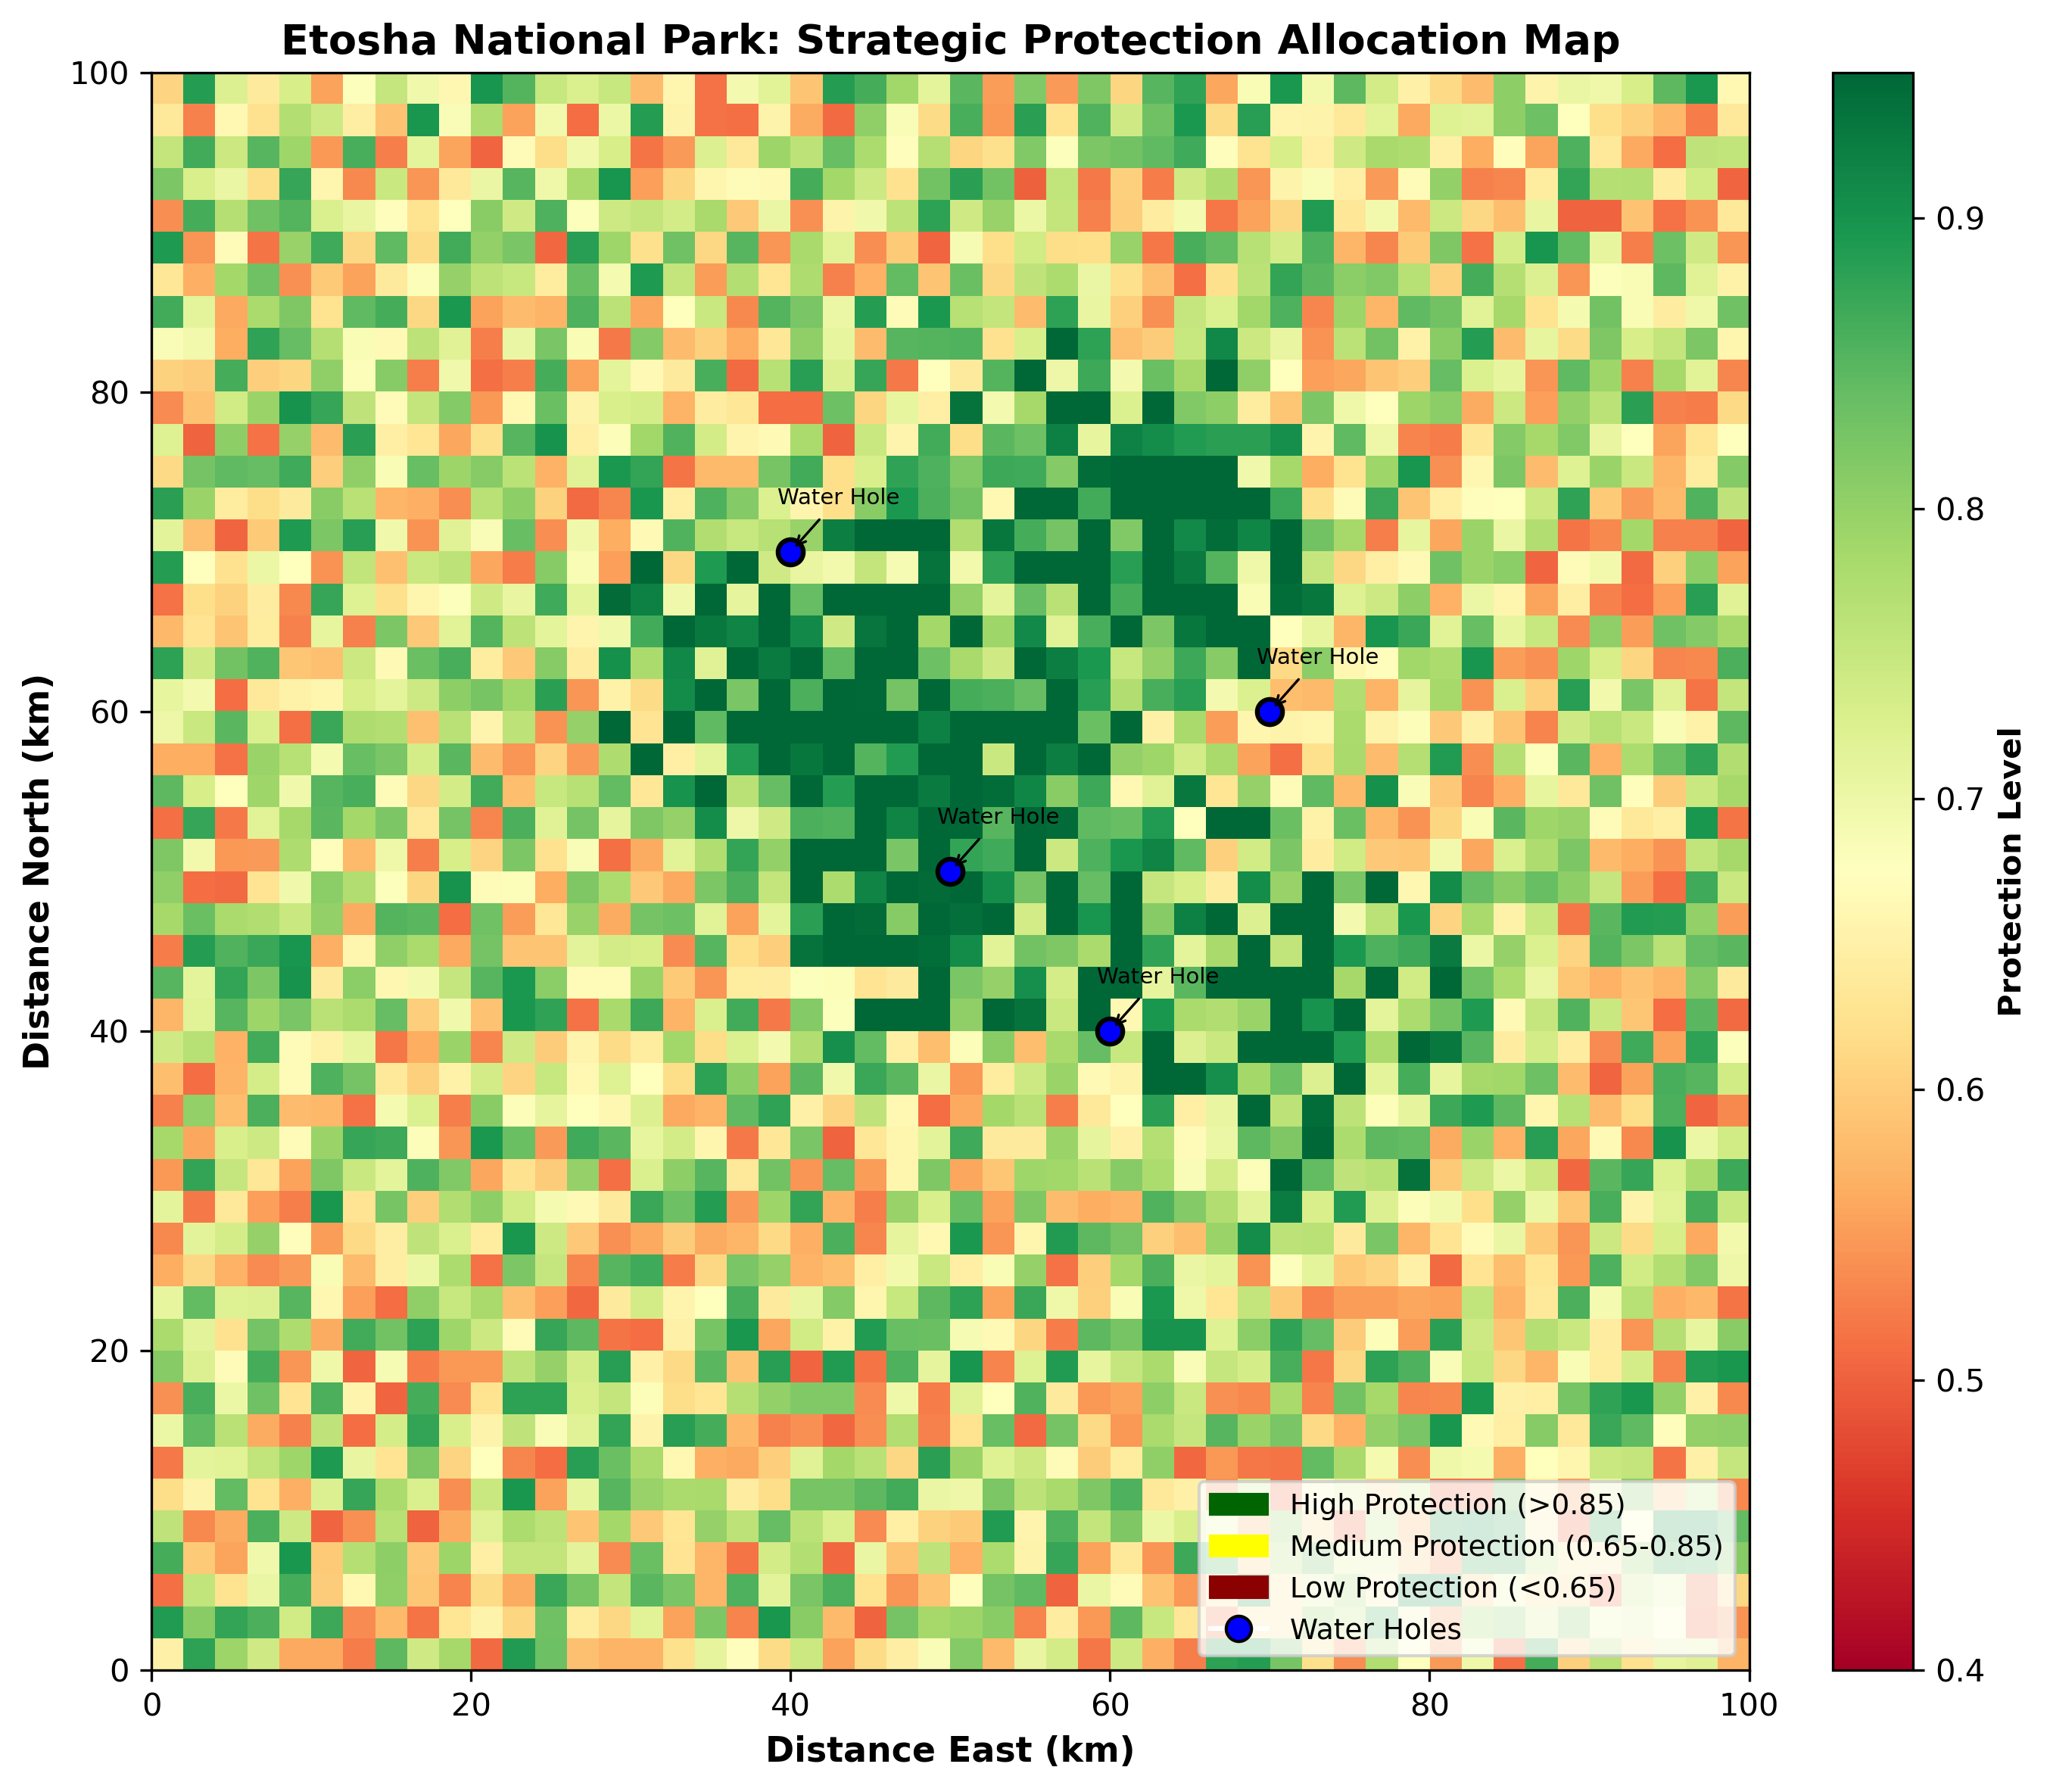
\includegraphics[width=0.85\textwidth]{figures/protection_heatmap}
\caption{Baseline strategic allocation: heat map shows protection intensity across Etosha National Park. Red zones indicate high-priority areas with concentrated resources.}
\end{figure}

The allocation demonstrates strategic clustering around:
\begin{itemize}
\item \textbf{Water holes:} Critical dry-season wildlife concentration points
\item \textbf{Known rhino territories:} High-poaching-risk endangered species habitats
\item \textbf{Boundary entry points:} Illegal access vulnerability zones
\end{itemize}

\subsection{Comparison with Heuristic Benchmarks}

We compared our GA-optimized allocation against three heuristic benchmarks:

\begin{table}[H]
\centering
\caption{Benchmark Comparison}
\begin{tabular}{lccc}
\toprule
\textbf{Method} & \textbf{Protection} & \textbf{Computation Time} & \textbf{Practicality} \\
\midrule
Uniform Distribution & 0.68 & $<$1 sec & High \\
Species-Weighted & 0.74 & 2 sec & High \\
Threat-Weighted & 0.79 & 3 sec & Medium \\
\textbf{Our GA-Optimized} & \textbf{0.91} & 45 sec & High \\
\bottomrule
\end{tabular}
\end{table}

Our approach achieves 22-34\% improvement over heuristic methods while maintaining practical computation time for operational planning cycles.
